
\section{Introduction}
The principles of electrostatics play a crucial role in our
understanding of everyday phenomena such as the formation of
lightning in weather storms to the operation of electrical devices
such as capacitors which make our stereos, computers, TVs', and
many other electrical systems work.  In this lab we will learn
about these principles by performing a few simple experiments that
will demonstrate concepts such as charge production, charge
conservation, electric fields, and electric potentials (for a
comprehensive overview of these subjects refer to your text book
by Serway, Chapters 23, 24, and 25).

\section{Theory}
\subsection{Electric Charge}
At one time or another we have all experienced what happens when
on a dry day, we close our car door, or we walk across a rug and
then touch a door knob.  The little shock-like feeling is a result
of an electrostatic imbalance created between us and the
environment.   This imbalance is due to the build-up of electric
charge in our bodies and the objects we come in contact with. The
amount of charge that can be acquired by a particular object
depends on its electrical properties.

Charge is a quantity measured in units of coulomb denoted by C. It
is a conserved quantity meaning that when we speak about charges
acquired by objects what we really should be saying is that
charges have been moved from one place to another, as to create
some imbalance of charge in that object.  We cannot create nor
destroy charge.

\subsection{Coulomb's Law}
Charged objects exert forces on each other.  We say that like
charges repel while unlike charges attract.  Thus there are two
kinds of charges; we call one positive, the other negative.  It is
possible to quantify this force by a mathematical relation known
as {\bf{Coulomb's Law}} which depends on the magnitudes of the
charges in question, their separation, and a constant:

\begin{equation}
F=\frac{1}{4\pi\epsilon_o}\frac{Q_1Q_2}{r^2} \label{CL}
\end{equation}

The equation above is the magnitude of the force between
two charges of magnitude $Q_1$ and $Q_2$ with $r$ being their
separation as shown in figure \ref{fig:electro:es1}.  The constant of
proportionality with units is given by:
\begin{eqnarray*}
\frac{1}{4\pi\epsilon_o}=8.99\times 10^9 ~{\rm N \cdot
\frac{m^2}{C^2}}.
\end{eqnarray*}

\begin{figure}[!htb]
\centering
\epsfxsize=6cm \includegraphics[scale=0.4]{1_electrostatics/es1.eps}
\caption{Two charges separated by a distance $r$.}
\label{fig:electro:es1}
\end{figure}

\subsection{Electric Field}
Imagine that the two charges in figure \ref{fig:electro:es1} are positive, and
that $Q_1$ is stationary at the origin.  Lets assume that at our
disposal is a device that could measure the force between these
two charges. If we move $Q_2$ in space, than according to
Eq.~(\ref{CL}) our device should measure different values for the
magnitude of the force as well as its direction at different
points. Thus we can think of $Q_2$ as being a test charge for
determining the force on a charge at some point in space. Plotting
these different vectors in space would result in a vector field
that describes the force on a test charge (see figure {\ref{es2}).
In light of this it is possible to write the force on a charge as:
\begin{equation}
{\mathbf{F}}=Q{\mathbf{E}}\label{ef}.
\end{equation}

$\mathbf{E}$ is called the electric field which is defined to be
the force per unit charge.  It too is a vector which points in the
direction of the electric force, or opposite to it (depending on the sign of the test charge $Q$), and may be thought of as a field
in space giving rise to forces on charges.  Now, the interaction
among charges can be looked at as one mediated by a field.

In reality one usually encounters not point charges but
continuous distribution of charges which make the concept of an
electric field very useful in determining the forces by use of
Eq.~(\ref{ef}).
\begin{figure}[!htb]
\centering
\epsfxsize=6cm 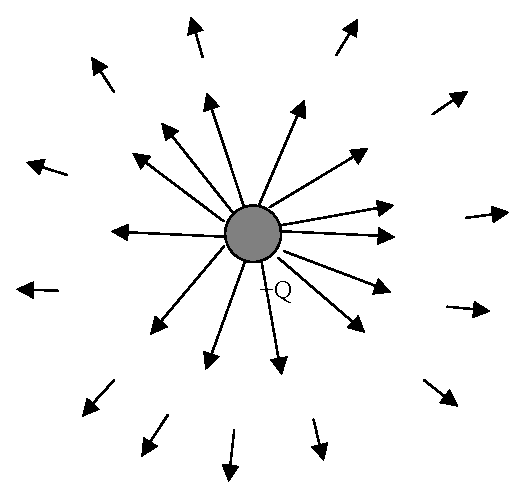
\includegraphics[scale=0.4]{1_electrostatics/es2.eps}
\caption{Electric field lines due to a point charge.}
 \label{es2}
\end{figure}

\subsection{Gauss' Law}

Determining the electric field for an arbitrary charge
distribution in space can sometimes be a very difficult task.
However, for charge distributions which possess certain
symmetries this task can become quite easy by the use of Gauss'
Law which is given by the following mathematical statement:
\begin{equation}
\oint{\mathbf{E}}\cdot\mathrm{d}{\mathbf{A}}=\frac{Q_{enc}}{\epsilon_o}.\label{GL}
\end{equation}

The equation above is a surface integral of the electric field
dotted with a  differential surface element over a Gaussian
surface which encloses a charge of magnitude $Q_{enc}$.  The left
side of Eq.~(\ref{GL}) is called the {\bf{electric flux}} which
can be thought of as measure of `flow' of the electric field
through the surface enclosing the charge.  Thus for a flux equal
to zero there should be no net charge inside the Gaussian surface.

By choosing the surface appropriately the integral of
Eq.~(\ref{GL}) can be performed to solve for $\mathbf{E}$.  Let's
use it to find the electric field due to a very thin rod carrying
a uniform positive charge (fig.~\ref{es3}).  Positioning the rod
along the $z$ axis, figure \ref{es3} suggests cylindrical symmetry
in which the electric field is constant along a surface of a
cylinder with a radius $r$, and a height $h$.  In this case we may
apply equation (\ref{GL}) over the surface of the cylinder which
is now our Gaussian surface:
\begin{eqnarray*}
\oint{\mathbf{E}}\cdot\mathrm{d}{\mathbf{A}}& = &
E\int\mathrm{d}A\\
& = & E2\pi r h= \frac{Q_{enc}}{\epsilon_{o}}.
\end{eqnarray*}



Note that in the second step we have used the fact that $E$ is
constant along the Gaussian surface enabling us to pull it out of
the integral.  The normal to the surface element is along the same
direction of the field, so that their dot product is just the
multiplication of their amplitudes.\\




Before completing the calculation we have to find what is
$Q_{enc}$.  We may define a quantity denoted by $\lambda$ to be a
charge density, or in this case a charge per unit length, so that
$Q_{enc}$ may be given by:
\begin{eqnarray*}
Q_{enc}= \lambda h.
\end{eqnarray*}

\noindent With this the electric field due to a line of charge is
given by:
\begin{equation}
E= \frac{\lambda}{2\pi\epsilon_o r}.\label{line}
\end{equation}

\begin{figure}[!htb]
\centering
\epsfxsize=6cm \includegraphics[scale=0.4]{1_electrostatics/es3.eps}
\caption{A Gaussian surface due to a line of charge}
 \label{es3}
\end{figure}



\subsection{Electric Potential}
Since an electric charge experiences a force in the presence of an
electric field then a charge initially at rest will start to move
under the influence of the field, and thus will gain kinetic
energy.  This means that the force which arises due to the field
will do work on the charged particle.  You may have noticed that
the electrical force is very similar in form to that of a
gravitational force, where, in the gravitational law, we use masses
instead of charges and we don't consider repulsion among masses.
Nonetheless the dependence on $r$ and the way we define the
direction of the force are exactly the same. From our mechanics
course we remember that the gravitational force is conservative,
and we therefore can convince ourselves that the electrical force
is conservative as well.  We can now use conservation of energy
which tells us that the change in potential energy is equal to the
negative change in kinetic energy, or simply put:

\begin{equation}
W=U_i-U_f
\end{equation}

Applying this equation with the definition of work, and
Eq.~(\ref{ef}) we get

\begin{equation}
W_{i\rightarrow f}=\int^f_i
{\mathbf{F}}\cdot\mathrm{d}{\mathbf{l}}=\int^f_i
Q{\mathbf{E}}\cdot\mathrm{d}{\mathbf{l}}.\label{pe}
\end{equation}

Dividing both sides by $Q$ (remembering that $Q$ is just a test
charge) the equation above can be written as:

\begin{eqnarray}
\frac{W_{i\rightarrow f}}{Q} =  \frac{U_i}{Q}-\frac{U_f}{Q} =
\int^f_i{\mathbf{E}}\cdot\mathrm{d}{\mathbf{l}}.\label{p}
\end{eqnarray}

The quantity $\frac{U}{Q}$ is called the {\bf{electric potential}}
denoted by V and is defined to be the potential energy per unit
charge. It is conventional to speak of an external force moving a
test charge in an electric field in which case it is the external
force doing the work and not the field.  This introduces a minus
sign in Eq.~(\ref{p}), and the potential difference of moving a
test charge from point $a$ to point $b$ is:

\begin{equation}
V_b-V_a=-\int^b_a{\mathbf{E}}\cdot\mathrm{d}{\mathbf{l}}.\label{fp}
\end{equation}

Let us apply this formula to find the electric potential in our
previous example of a very thin rod with positive charge.  If we
move a test charge from some point $a$ to some point $b$ radially
to-wards the rod we can use Eq.~(\ref{line}) together with
Eq.~(\ref{fp}) to get
\begin{eqnarray}
V_b-V_a & = &
-\frac{\lambda}{2\pi\epsilon_o}\int^{r_b}_{r_a}\frac{\mathrm{d}r}{r}
 =
 -\frac{\lambda}{2\pi\epsilon_o}\ln{\frac{r_b}{r_a}},\label{linev}
\end{eqnarray}
%where the minus sign in Eq.~(\ref{fp}) has been canceled since
%the displacement of the test charge opposes the direction of the electric field.\\
\vspace{1.2cm}


\noindent{\bf{Equipotential Surfaces}}

\noindent Moving a charge on a surface where no work is being done
by the electric field describes a charge moving on an
equipotential surface which is defined as a surface where the
potential is the same at every point.  Since no work is being done
on this surface it follows that the electric field has no
components parallel to it.  Thus, it is always the case that an
equipotential surface is perpendicular to the field.  Since every
point has a unique value for the potential it follows that
different equipotential surfaces can never intersect.\\


Finally, we note that Eq.~(\ref{fp}) can be written as
\begin{eqnarray*}
V_b-V_a=\int^b_a\mathrm{d}V=-\int^b_a{\mathbf{E}}\cdot\mathrm{d}{\mathbf{l}}.
\end{eqnarray*}

Assuming for simplicity that the displacement is only along the
$y$ axis, then the equation above can be written as
\begin{eqnarray*}
-\int^b_a\mathrm{d}V=\int^b_a E_y\mathrm{d}y.
\end{eqnarray*}

Since the limits of integration are arbitrary points it implies
that the integrands are equal, or simply put
\begin{equation}
E=-\frac{dV}{dy}.\label{efp}
\end{equation}

We could have done the same thing for the $x$ and $z$ components,
and since the potential $V$ is a function of all the coordinates
the equation above can be generalized to read
\begin{equation}
{\mathbf{E}}=-\nabla V,
 \label{ft}
\end{equation}

with $\nabla$ given by:
\begin{eqnarray*}
\nabla=\frac{\partial}{\partial x}\hat{i}+\frac{\partial}{\partial
y}\hat{j}+\frac{\partial}{\partial z}\hat{k}
\end{eqnarray*}

Since potentials are usually easier to calculate and measure than
electric fields, Eq.~({\ref{ft}) provides a convenient way for
finding the electric field.



\section{Apparatus}
Figure \ref{es5} shows the apparatus to be used in the first part
of the lab.

\begin{figure}[!htb]
\centering
\epsfxsize=16cm 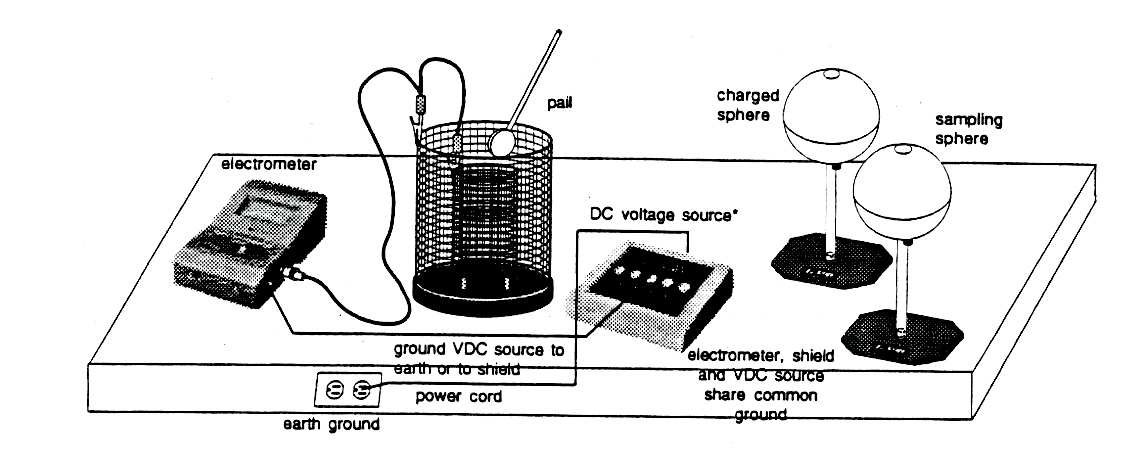
\includegraphics[scale=0.8]{1_electrostatics/Electrostatics.eps}
\caption{Apparatus (left to right): Electrometer, ice
pail, proof-plane and charge producers, electrostatic source, and
conducting spheres.}
 \label{es5}
\end{figure}

\subsection{The {\it Pasco} ES-9077 Electrostatics Voltage Source}
This is a high voltage, low current power supply designed
exclusively for experiments in electrostatics.  It has outputs at
30 V, 1000 V, 2000 V, 3000 V, and a ground connection.


\subsection{The {\it Pasco} ES-9078 Electrometer}

This is a voltmeter used for direct measurements of voltage
and indirect measurements of current and charge. \\

\fbox{\parbox{8cm}{\bf{Never use the electrometer for measuring
potentials more
than 100 V.\\
Never touch the input leads until you have grounded yourself to an
earth ground.}}} \vspace{0.2cm}

\noindent {\bf{Operation}}\\
$\bullet$ Before turning on the electrometer, check that the meter
reads zero.  If not, turn the Mechanical Zero Adjust screw,
located just below the meter face, until it does.\\
$\bullet$ Connect the test lead to the input connector of the
electrometer.\\
$\bullet$ Connect the ground post of the electrometer to an earth
ground by connecting to the COM on the Electrostatic Voltage Source, and plugging the AC
adapter to a wall outlet.\\
$\bullet$ Push the Power button ON.  One of the range switch LEDs
will blink twice in quick succession.\\
$\bullet$ To zero the meter, press the ZERO button.  You are now
ready to use the electrometer to measure charge, current or
voltage.\\
$\bullet$ Set the range switch to the desired voltage range.  The
range setting refers to the voltage input required to produce a
full scale meter deflection.  Between measurements, always press
the Zero button to discard all charge from the electrometer.

\subsection{The {\it Pasco} ES-9042A Faraday Ice Pail}
This apparatus was originally designed by Michael Faraday.  It
works on the principle that any charge placed inside a conducting
surface will induce an equal charge on the outside of the surface.
The ice pail is a good method for sampling charges and charge
distributions.

The Pasco Ice Pail consists of two wire mesh cylinders, one inside
the other, mounted on a molded plastic bottom.  The outer cylinder
is called the shield, and when grounded helps eliminate stray
charges and AC fields.  The inner cylinder is the actual pail
which is mounted on insulated rods.  When a charged object is
placed inside the pail, but without touching it, a charge of the
same magnitude is induced on the outside of the pail.  An
electrometer connected between the pail and shield will detect a
potential difference which is an indirect measurement of charge.


\subsection{The {\it Pasco} ES-9075A Charge Producers and Proof Planes}
\noindent {\bf{Charge Producers}}\\
The charge producers consist of two wands,
one with blue and one with white material attached to a conductive
disk. If the blue and white surfaces are briskly rubbed together,
the white surface acquires a positive charge, and the blue surface
acquires a negative charge.  Some guidelines are important to
remember when
using the charge producers.\\

\noindent $\bullet$ To get rid of excess charge and to neutralize
the charge
producers touch the conductive disk to ground. \\
$\bullet$ Avoid touching the neck during use.  The oils from your
hands will provide a path for charges to leak off.\\

\noindent {\bf{The Proof Plane}}\\
The proof plane is an aluminum covered conductive disk attached to
an insulated handle.  It is used to sample the charge density on
charged conductive surfaces.  A Faraday Ice Pail can then be used
to measure the charge density on the proof plane.  By touching the
proof plane to a surface, the proof plane will acquire a similar
charge distribution to the section of the surface that is touched.

When a proof plane is touched to a conductive surface, the proof
plane becomes part of the conductive surface.  Therefore it's
always best to touch the proof plane to the conductor in such a
way as to minimize the distortion of the shape of the surface. For
example, if the surface is a conducting sphere then the proof plane
needs to be touched with its large surfaces tangent to the surface
of the sphere.


\subsection{The {\it Pasco} ES-9059 13-cm Spheres}
The conductive spheres are used to store electrical charge.  The
spheres are composed of plastic resin mold plated with a copper
base, outer plating of non-sulphur brite nickel, with final
plating of chrome.  The spheres are mounted on insulating rods,
attached to a support base.  Each sphere has a thumb nut on the
lower half that can be used for attaching a ground cable or a lead
from a power supply.  The spheres and insulating rods should be
kept free of dirt, grease, and fingerprints to minimize leakage of
charge from the spheres.

\subsection{The {\it Pasco} High Resistance Paper and Conductive Ink}
This apparatus will be used in the second part of the lab to
measure voltage at different points in space due to long lines of
charge.  The conductive ink painted on a high resistance paper
will be connected to a power source.  This will create a potential
distribution across the paper which will be measured by an
electrometer.

The set up (see figure \ref{es4}) of this apparatus in the
experiment to follow will consist of two long parallel lines
drawn by conductive ink on the high resistance paper.  The lines
are separated by some distance $d$ which is relatively smaller
than their length $L$. Now we can connect both lines to a static
power source; one to the positive end, the other to the negative
end. This will cause the lines to be charged with opposite
polarities creating a potential difference across them. If these
lines are drawn uniformly and the measurements are done close to
the center of the lines (we want to stay close to the center, since
near the edges the field deviates from Eq.~(\ref{linev})) then
using Eq.~({\ref{linev}) we can find the potential between these
two lines on the plane of the paper.

\begin{figure}[!htb]
\centering
\epsfxsize=12cm 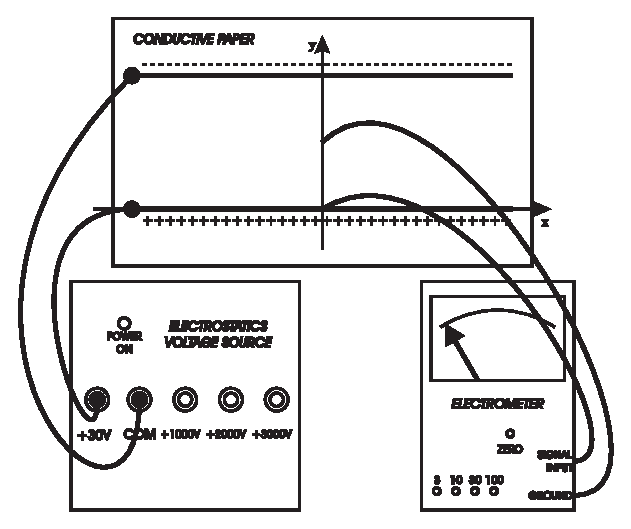
\includegraphics[scale=0.7]{1_electrostatics/es4.eps} 
\caption{High resistance paper and conductive ink.} \label{es4}
\end{figure}

Assume we want to know the potential at a point along the $y$ axis
(see figure \ref{es4}) between the two lines of charge. Using
Eq.~({\ref{linev}) we can sum the potential due to the positive
line and the negative line respectively to get
\begin{eqnarray*}
V(y)=
\frac{\lambda}{2\pi\epsilon_o}\big(\ln{\frac{r_o}{y}}-\ln{\frac{d-r_o}{d-y}}\big).
\label{exv}
\end{eqnarray*}

The radius $r_o$ is a reference point with respect to which we
measure the potential at a point on the $y$ axis located above the
positive line of charge.  Choosing our reference point $r_o$ to be
$\frac{d}{2}$ the equation above reduces to the following:

\begin{equation}
V(y)=\frac{\lambda}{2\pi\epsilon_o}\ln{\frac{d-y}{y}},\label{2lines}
\end{equation}

\noindent which gives the potential between the two lines at a
point in the same plane of the lines.  Note that for our
experiment Eq.~(\ref{2lines}) is not valid at the points $y=0$, or
$y=d$ since this equation was derived for infinitely long thin
lines of charge which have no thickness.  Such conditions are hard
if not impossible to obtain in lab, meaning our lines of charge
will be finite both in length and in thickness.

\vfill
\clearpage
%$$
%$$
%\newpage

\renewcommand{\thesection}{\thechapter.W}
\section{Electrostatics Worksheet}
\noindent{\bf\Large Name:}~\rule{5.0cm}{0.1mm}~~~~~~~ {\bf\Large
Day/Time}~\rule{3cm}{.1mm}\\
{\bf\Large Partner's Name:}~\rule{6cm}{.1mm}\\
\noindent
\subsection{In-Lab Procedure}

All measurements with the electrometer should include units and
uncertainties in the space provided. Whenever you are not using
the power supply you should turn it off.

\subsubsection{Faraday Ice Pail and Charge Production}
The purpose of this experiment is to investigate the relation
between the charge induced on the ice pail by a charged object
placed in the ice pail, and the charge of the object.

\noindent Before beginning the experiment the pail and
electrometer must be momentarily grounded.  To do this use the
black wire with two alligator clips toward one end; one positive
(red) the other negative (black).  Connect the electrometer's
negative clip to the shield, and the positive clip to the ice pail
as shown in figure \ref{es5}.  Connect the other end (called a
BNC) to the electrometer SIGNAL INPUT.  Also connect the earth
ground of the electrometer to the COM input of the electrostatic
source, and make sure the source is connected to a wall outlet.
Press the {\it Zero} button of the electrometer. This should
remove all stray charges from the pail and the electrometer
should read zero. You should also ground yourself to eliminate
stray charges from your body by touching the
ice pail when the {\it Zero} button is pressed.\\

\noindent {\bf A: Charging by Induction vs. Charging by Contact}\\
\noindent Set the voltage range of the electrometer to $100$V. Start with
this scale for every new measurement you perform, so that you don't destroy
the instrument with a high voltage. After you take an initial reading, adjust
the electrometer incrementally to the finest scale that will accomodate your
measurements. This will assure that you get the maximum precision. Do observe
that you may have to readjust the electrometer scale several times in today's
experiment.

\noindent Remove any stray charges on the charge producers by touching the
necks and handles to the shield of the ice pail while the {\it Zero} button is
pressed.  Avoid touching the necks of the charge producers with your hands
since oils on your hands will cause charge to leak in future use. 

\noindent Rub the white and blue
surfaces together to separate charges. Do this for about ten seconds.  After
this, place one of the charge producers far away so that it does not come in
contact with any of the ice pail surfaces.\\
\noindent While touching the grounded shield insert the other
charge producer into the ice pail all the way to the lower half of
the pail, but without letting it touch the pail.  Record the
electrometer reading below.\\ 

\vspace{1cm}

\hspace{4cm}$V_{1A}=$\rule{5.0cm}{.1mm}\\

%\vspace{1cm}

\noindent Remove the object and again record the electrometer
reading below (make sure that the handle never touches the pail
when removing the object).\\

\vspace{1cm}

\hspace{4cm}$V_{2A}=$\rule{5.0cm}{.1mm}\\

%\vspace{1.0cm}

\noindent Now, press the {\it Zero} button to remove any residual
charge.  Insert the object again, but this time let it touch the
ice pail.  Remove the object and record the voltage
reading.\\

\vspace{1cm}

\hspace{4cm}$V_{3A}=$\rule{5.0cm}{.1mm}\\

%\vspace{1cm}

\noindent Press the {\it Zero} button of the electrometer to
remove all charges and insert the object again into the ice pail
(again without touching the pail) and record
the voltage reading.\\

\vspace{1cm}

\hspace{4cm}$V_{4A}=$\rule{5.0cm}{.1mm}\\

%\vspace{1cm}

%\newpage

\noindent{\bf{B: Conservation of charge}}\\
\noindent Starting with the uncharged producers, rub the blue and
white producers together.  Keep them in your hands, without
letting them touch each other or the ice pail. Insert the charge
producers one at a time into the pail and record the voltage readings.\\


\vspace{0.5cm}

\hspace{4cm}$V_{1B}=$\rule{5.0cm}{.1mm}

\vspace{0.5cm}

\hspace{4cm}$V_{2B}=$\rule{5.0cm}{0.1mm}

\vspace{0.5cm}
 \noindent Remove all charge from the charge producers by grounding
 them (don't forget to ground the necks of the wands as well).
 Insert both charge producers into the pail and record the voltage reading.\\

\vspace{1cm}
  \hspace{4cm}$V_{3B}=$\rule{5.0cm}{.1mm}
\vspace{0.5cm}

 \noindent Rub them inside the pail without touching the sides of the ice pail. Record the voltage
 reading.\\

\vspace{1.0cm}
  \hspace{4cm}$V_{4B}=$\rule{5.0cm}{.1mm}

\vspace{0.5cm}
 \noindent Remove one of the charge producers and
record the voltage reading.\\

\vspace{1cm}
  \hspace{4cm}$V_{5B}=$\rule{5.0cm}{.1mm}

\vspace{0.5cm}


\noindent Remove the charge producer from the pail and insert the
other into the ice pail.  Record the voltage reading.



\vspace{1cm}
  \hspace{4cm}$V_{6B}=$\rule{5.0cm}{.1mm}

%\vspace{1cm}

\subsubsection{Charge Distribution}
\noindent The purpose of this procedure is to investigate the way
charge is distributed over a surface, by measuring variations
of charge density.\\
Make sure the ice pail is properly grounded with the shield
connected to earth ground of the electrometer, and the 
electrometer is connected to the COM  of the voltage source.
Make sure the voltage source is connected to a wall outlet.\\
\noindent Place the two aluminum spheres about 50 cm apart.
Connect one of the spheres to the $1000$V DC outlet of the
electrostatic voltage source.  This sphere will be used as a
charging body.\\
\noindent Momentarily ground the other sphere(NOT THE ONE
CONNECTED TO THE VOLTAGE SOURCE) by touching the sphere with the
shield of the pail. \\
\noindent Using the proof plane sample the uncharged sphere by
touching it in few places (on the side close to the other sphere,
on the side far from the other sphere, and midway between these two
points on the sphere), and then placing the proof plane in the ice
pail to read the voltage. Note that when touching the sphere with
the proof plane it is best to minimize any distortion of the
surface area of the sphere by touching the proof plane flat
against
the surface.  You must also remember that between samplings of the uncharged 
sphere the proof plane must not be grounded.  Record the voltage readings.\\

  \hspace{3.6cm} \textbf{close} }\hspace{2cm} \textbf{midway} \hspace{2.2cm} \textbf{far}\\

\vspace{1cm}
  \hspace{2cm}$V_{1C}=$\rule{2.5cm}{.1mm}\hspace{1cm}\rule{2.5cm}{.1mm}\hspace{1cm}\rule{2.5cm}{.1mm}

\vspace{1cm}

\noindent Bring the 1000V DC sphere close to the uncharged sphere
until they are approximately 1 cm apart.  Turn the voltage source
on and sample the sphere at the same points as before.  Record the
voltage readings.\\


\vspace{1cm}
  \hspace{2cm}$V_{2C}=$\rule{2.5cm}{.1mm}\hspace{1cm}\rule{2.5cm}{.1mm}\hspace{1cm}\rule{2.5cm}{.1mm}

\vspace{1cm}

\noindent Remove the 1000V DC sphere until it is at least 50 cm
away from the sampling sphere.  Again repeat the sampling at the
same points and record their values.

\vspace{3cm}
  
\hspace{2cm}$V_{3C}=$\rule{2.5cm}{.1mm}\hspace{1cm}\rule{2.5cm}{.1mm}\hspace{1cm}\rule{2.5cm}{.1mm}

\vspace{1cm}

\subsubsection{Electric Field and Electric Potential}
In this part of the experiment we will use the high resistance
paper and the conductive ink to create a charge distribution due
to two lines of charge with opposite polarities separated by
some distance. The purpose of this experiment is to see how the
electric potential and electric field vary with
this charge distribution.\\
Secure the high resistance paper (to be
supplied by your TA) to the cork board using thumb tacks. 
Note that the grid marked on the high resistance paper
is 1 cm $\times$ 1 cm. Measure the length of one of the lines 
$L$, and the separation distance between the two lines $d$ and 
record them below.\\

\vspace{1cm}
\hspace{3cm}$L=$\rule{2cm}{.1mm}\hspace{1cm}$d=$\rule{2cm}{.1mm}
\vspace{1cm}

\noindent Using the two cables which have at one end a connection
to the power supply, and at the other end holes, connect the COM of
the electrostatic source to one end of one line drawn by the
conductive ink.  Make this connection by securing the cable to the
wire with a thumb tack.  Make sure that the connection is made at
the ends of the lines (not center), and that the wires make
contact with the conductive ink. Connect the 30V output of the
power supply to the other line at the end by repeating the procedure above.\\

\noindent Using the red and black probe wires connected to the SIGNAL
INPUT, and ground connections of the electrometer respectively (in this
procedure the electrometer should not be grounded), place
the black probe in the center between the two lines. This
will be the voltage reference point for all measurements. Use
the second probe to measure the voltage with
respect to the reference point starting on the $y$ axis at 1 cm
above the positive line of charge going up in the positive $y$
direction.  Remember that the $y=0$ point on the $y$ axis is determined by
where the positive line of charge is located, while the positive y direction
is from the positive to the negative line of charge (see figure \ref{es4}).
When taking voltage measurements it is important that the probes be placed
perpendicular to the page and not slanted, as to minimize the distortion of
the charge distribution across the paper. Make your measurements in 1 cm
increments and record the value of the voltage in table \ref{tes1}
for each distance.  Your last measurement should be made 1 cm below the top
line which is the negative line of charge (see figure \ref{es4}). %neel

\begin{table}
\hspace{2cm}\begin{tabular}{|c|c|}\hline
\hspace{2cm} $V$ \hspace{2cm} & \hspace{2cm} $y$ \hspace{2cm} \\
\hline
\hspace{4cm} & \hspace{4cm} \\
\hline
\hspace{4cm} & \hspace{4cm} \\
\hline
\hspace{4cm} & \hspace{4cm} \\
\hline
\hspace{4cm} & \hspace{4cm} \\
\hline
\hspace{4cm} & \hspace{4cm} \\
\hline
\hspace{4cm} & \hspace{4cm} \\
\hline
\hspace{4cm} & \hspace{4cm} \\
\hline
\hspace{4cm} & \hspace{4cm} \\
\hline
\hspace{4cm} & \hspace{4cm} \\
\hline
\end{tabular}
\caption {Voltage and distance measurements.} \label{tes1}
\end{table}


\noindent Now do the following:\\
$a)$ Plot $V$ vs. $\ln\big({\frac{d-y}{y}}\big)$ in Kaleidagraph
with error bars and units.  All partners must have their own
plots. Show your
work in finding $\bigtriangleup\left(\ln{\big(\frac{d-y}{y}\big)}\right)$ here:\\
\vspace{8cm}\\
\noindent$b)$ Record the slope and intercept in table~\ref{tes2}
with units and uncertainties.\\
\begin{table}
\hspace{2cm}\begin{tabular}{|c|c|}\hline
\hspace{1cm} Slope \hspace{1cm} & \hspace{1cm} Intercept \hspace{1cm} \\
\hline
\hspace{4cm} & \hspace{4cm}\\
\hline
\end{tabular}
\caption{Slope and Intercept} \label{tes2}
\end{table}

 \noindent Finally place the probe (not the one at
the reference point) midway between the two lines.  Move the probe
1 cm to the right and 1 cm to the left along the $x$ axis with
respect to this point. Do you see any appreciable change in voltage? \\
What can you say about this line on which the probe moved?
\vspace{2cm}

\subsection{Pre-Classroom Check List}
\noindent This check list is intended to be a guide for you to
prepare yourself for the classroom work.  You cannot come back
to lab during this hour, collaborate with colleagues, nor hand in
the worksheet late.  Make sure you have completed everything.
\subsubsection{Pre-classroom Check List}
$\bigcirc$ \hspace{1cm} Voltages $V_{1A}$ through $V_{3C}$ have
units and uncertainties.\\
$\bigcirc$ \hspace{1cm} Table \ref{tes1} completed with units and
uncertainties.\\
$\bigcirc$ \hspace{1cm} Table \ref{tes2} completed with units and
uncertainties.\\
$\bigcirc$ \hspace{1cm} Each student should have her/his own plot
and worksheet.

\subsection{In-Classroom Calculations \& Analysis}
{\bf{Faraday Ice Pail and Charge Production}}\\
\vspace{0.2cm}

\noindent {\bf A: Charging by Induction vs. Charging by Contact}\\
 \noindent Using your data only from this part of the
experiment answer the following questions:\\

\noindent Explain why was there a potential difference between the
pail and the shield only while the charged object was inside
(where the object did not touch the pail).\\
\vspace{5cm}


\noindent Explain why after touching the pail with the charged
object there appeared a permanent potential difference between the pail and the shield.\\
\vspace{5cm}

\noindent Explain why there was again a potential difference after zeroing the electrometer and putting the object back inside. \\ %neel
\vspace{5cm}

\noindent{\bf{B: Conservation of charge}}\\
Using your data only from this part of the experiment answer the
following questions:\\
\noindent After placing the charged objects one at a time into the
pail what can you conclude about the magnitude of the charges, and
the relation between their polarity?\\

\vspace{5cm}

\noindent Was charge conserved in this experiment? Explain your answer.\\
\vspace{4cm}

\noindent {\bf{Charge Distribution}}\\
\noindent Using your data only from this part of the experiment
answer the
following questions:\\
\noindent What produced the charge distribution on the sphere that
you sampled?\\
\vspace{3cm}

\noindent What can you conclude about the charge distribution on a
metal sphere?
  Refer to both situations; first when the sampling
sphere was close to the charged sphere, and second when the
sampling sphere was far from the charged sphere.\\
 \vspace{3cm}

\vspace{0.4cm}

\noindent {\bf Electric Field and Electric Potential}\\
\noindent Using your data only from this part of the experiment
complete the
following:\\

\noindent Using the slope $a$ of your graph (given in table \ref{tes2}) and
Eq.~(\ref{exv}) calculate the charge per unit length $\lambda$.\\
\vspace{3.5cm}

\noindent Now calculate the total charge $Q$ that each
line of conductive ink carried.\\
\vspace{3.5cm}

\noindent Use Eq.~(\ref{efp}) together with Eq. (\ref{exv}) to
derive the theoretical expression for the electric field $E_{theo}$ between the
two lines of charge (no uncertainty).\\
\label{etheo}
\vspace{3.5cm}

\noindent Using this expression, find $E_{theo}$ at the point $\frac{d}{2}$, midway between the two lines of charge (no uncertainty).
\vspace{3cm}

\noindent From table \ref{tes1} use the two data points just above and below the mid-point (should be fourth and sixth data points $y_6=\frac{d}{2}+0.5$ cm and $y_4=\frac{d}{2}-0.5$ cm) to calculate an experimental value for the electric field at the midpoint between the two lines: %neel
\begin{eqnarray*}
E_{exp}=-\frac{\partial V}{\partial y}\approx-\frac{V_6-V_4}{y_6-y_4}=
\end{eqnarray*}
\vspace{3cm}

\noindent Compare $E_{exp}$ and $E_{theo}$. Since neither has any uncertainty, calculate the percentage deviation of $E_{exp}$ from $E_{theo}$ (the difference between them as a percentage of $E_{theo}$).\\ %neel

\vfill
{\Large End Worksheet}
\renewcommand{\thesection}{\thechapter.\arabic{section}}






